\section{Sujetos}
El departamento de deportes de la Universidad Rafael Land\'ivar, le proporcion\'o al investigador, la colaboraci\'on de todos los deportes (f\'utbol, voleibol, baloncesto, tenis, banda, zumba, atletismo, nataci\'on, taekwondo, tenis de mesa y animaci\'on).
\medbreak
El investigador tuvo que realizar filtros para seleccionar la poblaci\'on, descartando aquellos deportes que entrenaban en las federaciones nacionales de Guatemala (lugares externos a la Universidad Rafael Land\'ivar), entre ellos estaban: Atletismo, nataci\'on y tenis.
\medbreak
Por otro lado, el investigador apart\'o los deportes que se ejercitaban dentro de una cancha deportiva debido a la dificultad de colocar todos los materiales necesarios del proyecto para la toma de datos, por lo cual se elimin\'o los deportes de:  f\'utbol, voleibol y baloncesto.
\medbreak
Finalmente, el investigador ignor\'o los deportes de banda y zumba, ya que son actividades que se trabajan en conjunto con otros departamentos de la Universidad Rafael Landivar (Unidad de artes Land\'ivar). De modo que el investigador seleccion\'o los siguientes deportes:
\begin{itemize}
	\item \textbf{Tenis de mesa:} Deporte de raqueta que se juega sobre una mesa rectangular de manera individual o en parejas, con el fin objetivo de golpear una peque\~na pelota.
	\item \textbf{Animaci\'on:} Deporte grupal que combina la m\'usica y gimnasia, a partir de rutinas de baile que entusiasma un p\'ublico o evento deportivo.
	\item \textbf{Taekwondo:} Deporte individual basado en el arte marcial coreano moderno, que consiste en el uso de los pies, brazos y pu\~nos dentro de un combate.
\end{itemize}
\subsection{Primer tipo} \label{sj:1t}
Define la cantidad de sujetos que participaron en la colecta de los datos para la creaci\'on del modelo de reconocimiento del movimiento, a partir de tres fases distintas:
\begin{itemize}
	\item \textbf{Construcci\'on:} Atletas que construyeron el modelo de detecci\'on de los pasos requerido de un movimiento v\'alido.
	\item \textbf{Pruebas:} Muestra de usuarios que se emple\'o para el c\'alculo de los m\'argenes de  errores del modelo.
	\item \textbf{Validaci\'on:} Conjunto de deportistas que realizaron las pruebas al modelo en tiempo real.
\end{itemize}
\subsubsection{Equipo de animaci\'on de la Universidad Rafael Land\'ivar} \label{sj:1t:ani}
\begin{table}[H]
\begin{center}
\caption{Muestra del equipo de animadoras}
\label{tab:MuestraCheerleaders}
\begin{tabular}{lc}
\hline
\multicolumn{1}{|l|}{\textbf{Descripci\'on}} & \multicolumn{1}{l|}{\textbf{Cantidad}} \\ \hline
\multicolumn{1}{|l|}{Atletas para la construcci\'on del modelo} & \multicolumn{1}{c|}{6} \\ \hline
\multicolumn{1}{|l|}{Atletas para las pruebas del modelo} & \multicolumn{1}{c|}{1} \\ \hline
\multicolumn{1}{|l|}{Atletas para la validaci\'on del modelo} & \multicolumn{1}{c|}{2} \\ \hline
\multicolumn{1}{|r|}{Total de atletas} & \multicolumn{1}{c|}{9} \\ \hline
\textbf{Fuente:} Propia.
\end{tabular}
\end{center}
\end{table}
\subsubsection{Equipo de tenis de mesa de la Universidad Rafael Land\'ivar}\label{sj:1t:ten}
\begin{table}[H]
\begin{center}
\caption{Muestra del equipo de tenis de mesa}
\label{tab:MuestraTenis}
\begin{tabular}{lc}
\hline
\multicolumn{1}{|l|}{\textbf{Descripci\'on}} & \multicolumn{1}{l|}{\textbf{Cantidad}} \\ \hline
\multicolumn{1}{|l|}{Atletas para la construcci\'on del modelo} & \multicolumn{1}{c|}{5} \\ \hline
\multicolumn{1}{|l|}{Atletas para las pruebas del modelo} & \multicolumn{1}{c|}{1} \\ \hline
\multicolumn{1}{|l|}{Atletas para la validaci\'on del modelo} & \multicolumn{1}{c|}{3} \\ \hline
\multicolumn{1}{|r|}{Total de atletas} & \multicolumn{1}{c|}{9} \\ \hline
\textbf{Fuente:} Propia.
\end{tabular}
\end{center}
\end{table}
\subsubsection{Equipo de taekwondo de la Universidad Rafael Land\'ivar}\label{sj:1t:tae}
\begin{table}[H]
\begin{center}
\caption{Muestra del equipo de taekwondo}
\label{tab:MuestraTaekwondo}
\begin{tabular}{lc}
\hline
\multicolumn{1}{|l|}{\textbf{Descripci\'on}} & \multicolumn{1}{l|}{\textbf{Cantidad}} \\ \hline
\multicolumn{1}{|l|}{Atletas para la construcci\'on del modelo} & \multicolumn{1}{c|}{15} \\ \hline
\multicolumn{1}{|l|}{Atletas para las pruebas del modelo} & \multicolumn{1}{c|}{1} \\ \hline
\multicolumn{1}{|r|}{Total de atletas} & \multicolumn{1}{c|}{16} \\ \hline
\textbf{Fuente:} Propia.
\end{tabular}
\end{center}
\end{table}
\subsection{Segundo tipo} \label{sj:2t}
A continuaci\'on se muestra un organigrama de la estructura del departamento de deportes de la Universidad Rafael Land\'ivar, en ella se muestra todos los profesionales que aportaron en la investigaci\'on:
\begin{figure}[H]
	\caption{Organigrama del departamento de deportes de la Universidad Rafael Land\'ivar}
	\label{fig:orgDeportes}
	\centering
	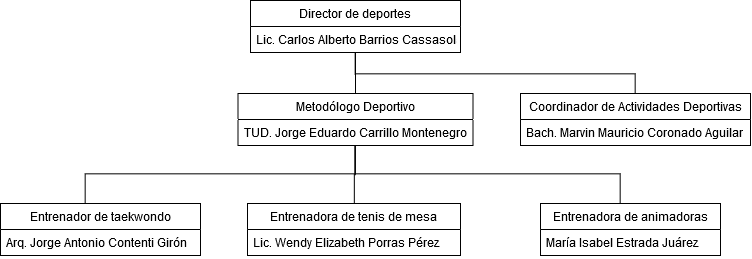
\includegraphics[width=450px,height=170px]{graphics/orgDeportes.png} \\
	\textbf{Fuente:} Propia.
\end{figure}
\subsection{Unidades de an\'alisis} \label{sj:ua}
Para el presente proyecto se utiliz\'o como referencia el manual de acondicionamiento de fuerza y prevenci\'on de lesiones  \cite{arbour2006strength}, la cual describe los movimientos ideales para el calentamiento  y estiramiento de una rutina. (ver secci\'on de anexos \ref{anx:warmup}).